\cleartoleftpage{}
\begin{figure}[p!]
  \begingroup
  \centering
  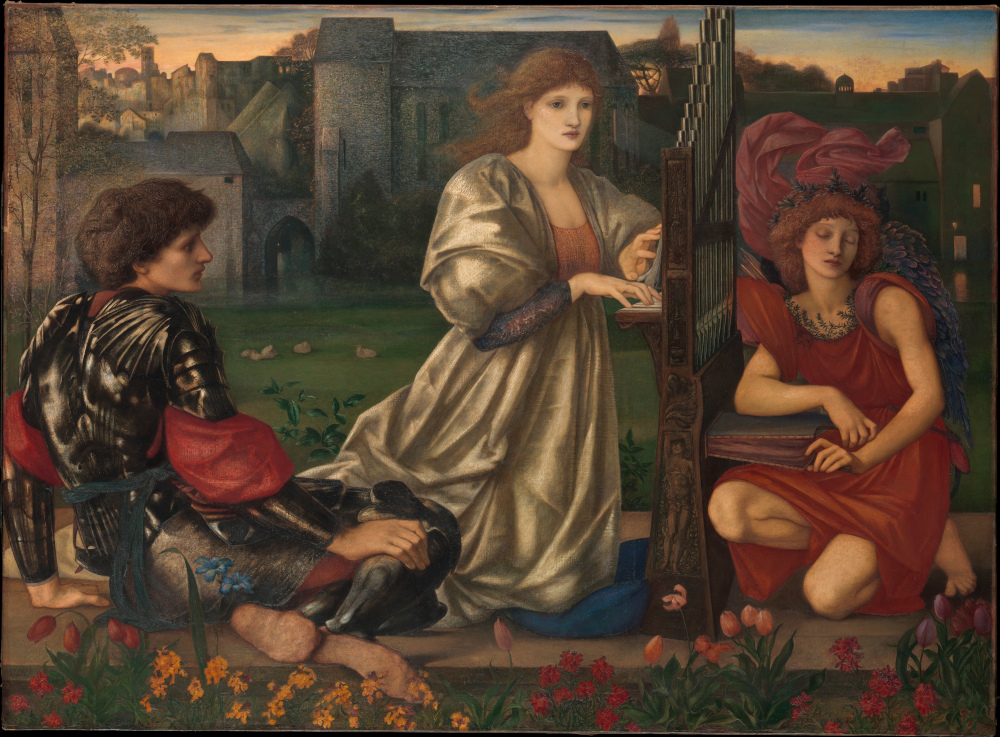
\includegraphics[keepaspectratio,width=\textwidth]{figures/The-Love-Song-Edward-Burne-Jones-small.jpg}
  \captionart{TheLoveSong}
  \label{fig:thelovesong}
\end{figure}

% Force float here
\clearpage{}
\thispagestyle{titleontop}
\chapter{Love and Its Objects}
{
\section{The Preface.}

\lettrine{T}{here} will not be wanting, I presume, one or other that will much
discommend some part of this treatise of love-melancholy, and object
(which \authorfootnote{4414}Erasmus in his preface to Sir Thomas More suspects of his)
that it is too light for a divine, too comical a subject to speak of
love symptoms, too fantastical, and fit alone for a wanton poet, a
feeling young lovesick gallant, an effeminate courtier, or some such
idle person. And 'tis true they say: for by the naughtiness of men it
is so come to pass, as \authorfootnote{4415} Caussinus observes, \li{ut castis auribus vox
amoris suspecta sit, et invisa}, the very name of love is odious to
chaster ears; and therefore some again, out of an affected gravity,
will dislike all for the name's sake before they read a word;
dissembling with him in \authorfootnote{4416}Petronius, and seem to be angry that
their ears are violated with such obscene speeches, that so they may be
admired for grave philosophers and staid carriage. They cannot abide to
hear talk of love toys, or amorous discourses, \li{vultu, gestu, oculis} in
their outward actions averse, and yet in their cogitations they are all
out as bad, if not worse than others.

\authorfootnote{4417}\li{Erubuit, posuitque meum Lucretia librum
Sed coram Bruto, Brute recede, legit.}

But let these cavillers and counterfeit Catos know, that as the Lord
John answered the Queen in that Italian \authorfootnote{4418}Guazzo, an old, a grave
discreet man is fittest to discourse of love matters, because he hath
likely more experience, observed more, hath a more staid judgment, can
better discern, resolve, discuss, advise, give better cautions, and
more solid precepts, better inform his auditors in such a subject, and
by reason of his riper years sooner divert. Besides, nihil in hac
amoris voce subtimendum, there is nothing here to be excepted at; love
is a species of melancholy, and a necessary part of this my treatise,
which I may not omit; operi suscepto inserviendum fuit: so Jacobus
Mysillius pleadeth for himself in his translation of Lucian's
dialogues, and so do I; I must and will perform my task. And that short
excuse of Mercerus, for his edition of Aristaenetus shall be mine,
\authorfootnote{4419}If I have spent my time ill to write, let not them be so idle as
to read. But I am persuaded it is not so ill spent, I ought not to
excuse or repent myself of this subject; on which many grave and worthy
men have written whole volumes, Plato, Plutarch, Plotinus, Maximus,
Tyrius, Alcinous, Avicenna, Leon Hebreus in three large dialogues,
Xenophon sympos. Theophrastus, if we may believe Athenaeus, lib. 13.
cap. 9. Picus Mirandula, Marius, Aequicola, both in Italian, Kornmannus
de linea Amoris, lib. 3. Petrus Godefridus hath handled in three books,
P. Haedus, and which almost every physician, as Arnoldus, Villanovanus,
Valleriola observat. med. lib. 2. observ. 7. Aelian Montaltus and
Laurentius in their treatises of melancholy, Jason Pratensis de morb.
cap. Valescus de Taranta, Gordonius, Hercules de Saxonia, Savanarola,
Langius, \etc{}, have treated of apart, and in their works. I excuse
myself, therefore, with Peter Godefridus, Valleriola, Ficinus, and in
\authorfootnote{4420}Langius' words. Cadmus Milesius writ fourteen books of love, and
why should I be ashamed to write an epistle in favour of young men, of
this subject? A company of stern readers dislike the second of the
Aeneids, and Virgil's gravity, for inserting such amorous passions in
an heroical subject; but \authorfootnote{4421}Servius, his commentator, justly
vindicates the poet's worth, wisdom, and discretion in doing as he did.

Castalio would not have young men read the Canticles\authorfootnote{4422}, because to
his thinking it was too light and amorous a tract, a ballad of ballads,
as our old English translation hath it. He might as well forbid the
reading of Genesis, because of the loves of Jacob and Rachael, the
stories of Sichem and Dinah, Judah and Thamar; reject the Book of
Numbers, for the fornications of the people of Israel with the
Moabites; that of Judges for Samson and Dalilah's embracings; that of
the Kings, for David and Bersheba's adulteries, the incest of Ammon and
Thamar, Solomon's concubines, \etc{} The stories of Esther, Judith,
Susanna, and many such. Dicearchus, and some other, carp at Plato's
majesty, that he would vouchsafe to indite such love toys: amongst the
rest, for that dalliance with Agatho,

\begin{latin}
\begin{verse}
Suavia dans Agathoni, animam ipse in labra tenebam;\\*
Aegra etenim properans tanquam abitura fuit.
\end{verse}
\end{latin}

For my part, saith \authorfootnote{4423}Maximus Tyrius, a great Platonist himself, me
non tantum admiratio habet, sed eliam stupor, I do not only admire, but
stand amazed to read, that Plato and Socrates both should expel Homer
from their city, because he writ of such light and wanton subjects,
Quod Junonem cum Jove in Ida concumbentes inducit, ab immortali nube
contectos, Vulcan's net. Mars and Venus' fopperies before all the gods,
because Apollo fled, when he was persecuted by Achilles, the \authorfootnote{4424}gods
were wounded and ran whining away, as Mars that roared louder than
Stentor, and covered nine acres of ground with his fall; Vulcan was a
summer's day falling down from heaven, and in Lemnos Isle brake his
leg, \etc{}, with such ridiculous passages; when, as both Socrates and
Plato, by his testimony, writ lighter themselves: quid enim tam distat
(as he follows it) quam amans a temperante, formarum admirator a
demente, what can be more absurd than for grave philosophers to treat
of such fooleries, to admire Autiloquus, Alcibiades, for their beauties
as they did, to run after, to gaze, to dote on fair Phaedrus, delicate
Agatho, young Lysis, fine Charmides, \li{haeccine Philosophum decent}? Doth
this become grave philosophers? Thus peradventure Callias,
Thrasimachus, Polus, Aristophanes, or some of his adversaries and
emulators might object; but neither they nor \authorfootnote{4425}Anytus and Melitus
his bitter enemies, that condemned him for teaching Critias to
tyrannise, his impiety for swearing by dogs and plain trees, for his
juggling sophistry, \etc{}, never so much as upbraided him with impure
love, writing or speaking of that subject; and therefore without
question, as he concludes, both Socrates and Plato in this are justly
to be excused. But suppose they had been a little overseen, should
divine Plato be defamed? no, rather as he said of Cato's drunkenness,
if Cato were drunk, it should be no vice at all to be drunk. They
reprove Plato then, but without cause (as \authorfootnote{4426}Ficinus pleads) for all
love is honest and good, and they are worthy to be loved that speak
well of love. Being to speak of this admirable affection of love (saith
\authorfootnote{4427}Valleriola) there lies open a vast and philosophical field to my
discourse, by which many lovers become mad; let me leave my more
serious meditations, wander in these philosophical fields, and look
into those pleasant groves of the Muses, where with unspeakable variety
of flowers, we may make garlands to ourselves, not to adorn us only,
but with their pleasant smell and juice to nourish our souls, and fill
our minds desirous of knowledge, \etc{} After a harsh and unpleasing
discourse of melancholy, which hath hitherto molested your patience,
and tired the author, give him leave with \authorfootnote{4428}Godefridus the lawyer,
and Laurentius (cap. 5.) to recreate himself in this kind after his
laborious studies, since so many grave divines and worthy men have
without offence to manners, to help themselves and others, voluntarily
written of it. Heliodorus, a bishop, penned a love story of Theagines
and Chariclea, and when some Catos of his time reprehended him for it,
chose rather, saith \authorfootnote{4429}Nicephorus, to leave his bishopric than his
book. Aeneas Sylvius, an ancient divine, and past forty years of age,
(as \authorfootnote{4430}he confesseth himself, after Pope Pius Secundus) indited that
wanton history of Euryalus and Lucretia. And how many superintendents
of learning could I reckon up that have written of light fantastical
subjects? Beroaldus, Erasmus, Alpheratius, twenty-four times printed in
Spanish, \etc{} Give me leave then to refresh my muse a little, and my
weary readers, to expatiate in this delightsome field, hoc deliciarum
campo, as Fonseca terms it, to \authorfootnote{4431} season a surly discourse with a
more pleasing aspersion of love matters: Edulcare vitam convenit, as
the poet invites us, curas nugis, \etc{}, 'tis good to sweeten our life
with some pleasing toys to relish it, and as \Pliny{} tells us, magna pars
studiosorum amaenitates quaerimus, most of our students love such
pleasant \authorfootnote{4432}subjects. Though Macrobius teach us otherwise,
\authorfootnote{4433}that those old sages banished all such light tracts from their
studies, to nurse's cradles, to please only the ear; yet out of
\Apuleius I will oppose as honourable patrons, Solon, Plato, \authorfootnote{4434}
Xenophon, Adrian, \etc{} that as highly approve of these treatises. On the
other side methinks they are not to be disliked, they are not so unfit.

I will not peremptorily say as one did \authorfootnote{4435}\li{tam suavia dicam facinora,
ut male sit ei qui talibus non delectetur}, I will tell you such pretty
stories, that foul befall him that is not pleased with them; \li{Neque
dicam ea quae vobis usui sit audivisse, et voluptati meminisse}, with
that confidence, as Beroaldus doth his enarrations on Propertius. I
will not expert or hope for that approbation, which Lipsius gives to
his Epictetus; \lit{the more I read, the more shall I covet to read}{pluris
facio quum relego; semper ut novum, et quum repetivi, repetendum}. I will not
press you with my pamphlets, or beg attention, but if you
like them you may. \Pliny{} holds it expedient, and most fit, \li{severitatem
jucunditate etiam in scriptis condire}, to season our works with some
pleasant discourse; Synesius approves it, \li{licet in ludicris ludere}, the
\authorfootnote{4436}poet admires it, \li{Omne tulit punctum qui miscuit utile dulci}; and
there be those, without question, that are more willing to read such
toys, than \authorfootnote{4437}I am to write: Let me not live, saith Aretine's
Antonia, If I had not rather hear thy discourse, \authorfootnote{4438}than see a play?
No doubt but there be more of her mind, ever have been, ever will be,
as \authorfootnote{4439}Hierome bears me witness. A far greater part had rather read
\Apuleius than Plato: Tully himself confesseth he could not understand
Plato's Timaeus, and therefore cared less for it: but every schoolboy
hath that famous testament of Grunnius Corocotta Porcellus at his
fingers' ends. The comical poet,\authorfootnote{4440}

\begin{latin}
\begin{verse}
---Id sibi negoti credidit solum dari,\\*
Populo ut placrent, quas fecissit fabulas,
\end{verse}
\end{latin}

made this his only care and sole study to please the people, tickle the
ear, and to delight; but mine earnest intent is as much to profit as to
please; non tam ut populo placerem, quam ut populum juvarem, and these
my writings, I hope, shall take like gilded pills, which are so
composed as well to tempt the appetite, and deceive the palate, as to
help and medicinally work upon the whole body; my lines shall not only
recreate, but rectify the mind. I think I have said enough; if not, let
him that is otherwise minded, remember that of \authorfootnote{4441}Maudarensis, he
was in his life a philosopher (as Ausonius apologiseth for him), in his
epigrams a lover, in his precepts most severe; in his epistle to
Caerellia, a wanton. Annianus, Sulpicius, Evemus, Menander, and many
old poets besides, did in scriptis prurire, write Fescennines,
Atellans, and lascivious songs; laetam materiam; yet they had in
moribus censuram, et severitatem, they were chaste, severe, and upright
livers.

\authorfootnote{4442}Castum esse decet pium poetam
Ipsum, versiculos nihil necesse est,
Qui tum denique habent salem et leporem.

I am of \Catullus{}' opinion, and make the same apology in mine own
behalf; \li{Hoc etiam quod scribo, pendet plerumque ex aliorum sententia et
auctoritate; nec ipse forsan insanio, sed insanientes sequor}. \li{Atqui
detur hoc insanire me; Semel insanivimus omnes, et tute ipse opinor
insanis aliquando, et is, et ille, et ego, scilicet.}\authorfootnote{4443} \li{Homo sum,
humani a me nihil alienum puto}:\authorfootnote{4444} And which he urgeth for himself,
accused of the like fault, I as justly plead, \authorfootnote{4445}\li{lasciva est nobis
pagina, vita proba est}. Howsoever my lines err, my life is honest,
\authorfootnote{4446}\li{vita verecunda est, musa jocosa mihi}. But I presume I need no
such apologies, I need not, as Socrates in Plato, cover his face when
he spake of love, or blush and hide mine eyes, as Pallas did in her
hood, when she was consulted by Jupiter about Mercury's marriage, quod,
super nuptiis virgo consulitur, it is no such lascivious, obscene, or
wanton discourse; I have not offended your chaster ears with anything
that is here written, as many French and Italian authors in their
modern language of late have done, nay some of our Latin pontificial
writers, Zanches, Asorius, Abulensis, Burchardus, \etc{}, whom \authorfootnote{4447}Rivet
accuseth to be more lascivious than Virgil in Priapeiis, Petronius in
Catalectis, Aristophanes in Lycistratae, Martialis, or any other pagan
profane writer, qui tam atrociter (\authorfootnote{4448}one notes) hoc genere
peccarunt ut multa ingeniosissime scripta obscaenitatum gratia castae
mentes abhorreant. 'Tis not scurrile this, but chaste, honest, most
part serious, and even of religion itself. \authorfootnote{4449}Incensed (as he said)
with the love of finding love, we have sought it, and found it. More
yet, I have augmented and added something to this light treatise (if
light) which was not in the former editions, I am not ashamed to
confess it, with a good \authorfootnote{4450}author, quod extendi et locupletari hoc
subjectum plerique postulabant, et eorum importunitate victus, animum
utcunque renitentem eo adegi, ut jam sexta vice calamum in manum
sumerem, scriptionique longe et a studiis et professione mea alienae,
me accingerem, horas aliquas a seriis meis occupationibus interim
suffuratus, easque veluti ludo cuidam ac recreationi destinans;
\authorfootnote{4451}Cogor---retrorsum
Vela dare, atque literare cursus
Olim relictos---

etsi non ignorarem novos fortasse detractores novis hisce
interpolationibus meis minime defuturos. \authorfootnote{4452}
And thus much I have thought good to say by way of preface, lest any
man (which \authorfootnote{4453}Godefridus feared in his book) should blame in me
lightness, wantonness, rashness, in speaking of love's causes,
enticements, symptoms, remedies, lawful and unlawful loves, and lust
itself, \authorfootnote{4454}I speak it only to tax and deter others from it, not to
teach, but to show the vanities and fopperies of this heroical or
Herculean love,\authorfootnote{4455}and to apply remedies unto it. I will treat of
this with like liberty as of the rest.

\authorfootnote{4456}Sed dicam vobis, vos porro dicite multis
Millibus, et facite haec charta loquatur anus.

Condemn me not good reader then, or censure me hardly, if some part of
this treatise to thy thinking as yet be too light; but consider better
of it; Omnia munda mundis, \authorfootnote{4457}a naked man to a modest woman is no
otherwise than a picture, as Augusta Livia truly said, and \authorfootnote{4458}\li{mala
mens, malus animus}, 'tis as 'tis taken. If in thy censure it be too
light, I advise thee as Lipsius did his reader for some places of
\Plautus{}, \li{istos quasi Sirenum scopulos praetervehare}, if they like thee
not, let them pass; or oppose that which is good to that which is bad,
and reject not therefore all. For to invert that verse of Martial, and
with Hierom Wolfius to apply it to my present purpose, \li{sunt mala, sunt
quaedam mediocria, sunt bona plura}; some is good, some bad, some is
indifferent. I say further with him yet, I have inserted
(\authorfootnote{4459}\li{levicula quaedam et ridicula ascribere non sum gravatus,
circumforanea quaedam e theatris, e plateis, etiam e popinis}) some
things more homely, light, or comical, litans gratiis, \etc{} which I
would request every man to interpret to the best, and as Julius Caesar
Scaliger besought Cardan (si quid urbaniuscule lusum a nobis, per deos
immortales te oro Hieronyme Cardane ne me male capias). I beseech thee,
good reader, not to mistake me, or misconstrue what is here written;
Per Musas et Charites, et omnia Poetarum numina, benigne lector, oro te
ne me male capias. 'Tis a comical subject; in sober sadness I crave
pardon of what is amiss, and desire thee to suspend thy judgment, wink
at small faults, or to be silent at least; but if thou likest, speak
well of it, and wish me good success. Extremum hunc Arethusa mihi
concede laborem.\authorfootnote{4460}

I am resolved howsoever, velis, nolis, audacter stadium intrare, in the
Olympics, with those Aeliensian wrestlers in Philostratus, boldly to
show myself in this common stage, and in this tragicomedy of love, to
act several parts, some satirically, some comically, some in a mixed
tone, as the subject I have in hand gives occasion, and present scene
shall require, or offer itself.

%SUBSECT. II.-_Love's Beginning, Object, Definition, Division_.
\section{Love's Beginning, Object, Definition, Division.}

\lettrine{L}{ove}'s limits are ample and great, and a spacious walk it hath, beset
with thorns, and for that cause, which \authorfootnote{4461}Scaliger reprehends in
Cardan, not lightly to be passed over. Lest I incur the same censure, 1
will examine all the kinds of love, his nature, beginning, difference,
objects, how it is honest or dishonest, a virtue or vice, a natural
passion, or a disease, his power and effects, how far it extends: of
which, although something has been said in the first partition, in
those sections of perturbations (\authorfootnote{4462} for love and hatred are the
first and most common passions, from which all the rest arise, and are
attendant, as Picolomineus holds, or as Nich. Caussinus, the primum
mobile of all other affections, which carry them all about them) I will
now more copiously dilate, through all his parts and several branches,
that so it may better appear what love is, and how it varies with the
objects, how in defect, or (which is most ordinary and common)
immoderate, and in excess, causeth melancholy.

Love universally taken, is defined to be a desire, as a word of more
ample signification: and though Leon Hebreus, the most copious writer
of this subject, in his third dialogue make no difference, yet in his
first he distinguisheth them again, and defines love by desire.

\authorfootnote{4463}Love is a voluntary affection, and desire to enjoy that which is
good. \authorfootnote{4464}Desire wisheth, love enjoys; the end of the one is the
beginning of the other; that which we love is present; that which we
desire is absent. \authorfootnote{4465}It is worth the labour, saith Plotinus, to
consider well of love, whether it be a god or a devil, or passion of
the mind, or partly god, partly devil, partly passion. He concludes
love to participate of all three, to arise from desire of that which is
beautiful and fair, and defines it to be an action of the mind desiring
that which is good. \authorfootnote{4466}Plato calls it the great devil, for its
vehemency, and sovereignty over all other passions, and defines it an
appetite, \authorfootnote{4467}by which we desire some good to be present. Ficinus in
his comment adds the word fair to this definition. Love is a desire of
enjoying that which is good and fair. \Austin{} dilates this common
definition, and will have love to be a delectation of the heart,
\authorfootnote{4468}for something which we seek to win, or joy to have, coveting by
desire, resting in joy. \authorfootnote{4469}Scaliger exerc. 301. taxeth these former
definitions, and will not have love to be defined by desire or
appetite; for when we enjoy the things we desire, there remains no more
appetite: as he defines it, Love is an affection by which we are either
united to the thing we love, or perpetuate our union; which agrees in
part with Leon Hebreus.

Now this love varies as its object varies, which is always good,
amiable, fair, gracious, and pleasant. \authorfootnote{4470}All things desire that
which is good, as we are taught in the Ethics, or at least that which
to them seems to be good; quid enim vis mali (as \Austin{} well infers)
dic mihi? puto nihil in omnibus actionibus; thou wilt wish no harm, I
suppose, no ill in all thine actions, thoughts or desires, nihil mali
vis; \authorfootnote{4471}thou wilt not have bad corn, bad soil, a naughty tree, but
all good; a good servant, a good horse, a good son, a good friend, a
good neighbour, a good wife. From this goodness comes beauty; from
beauty, grace, and comeliness, which result as so many rays from their
good parts, make us to love, and so to covet it: for were it not
pleasing and gracious in our eyes, we should not seek. \authorfootnote{4472}No man
loves (saith Aristotle 9. mor. cap. 5.) but he that was first delighted
with comeliness and beauty. As this fair object varies, so doth our
love; for as Proclus holds, Omne pulchrum amabile, every fair thing is
amiable, and what we love is fair and gracious in our eyes, or at least
we do so apprehend and still esteem of it. \authorfootnote{4473} Amiableness is the
object of love, the scope and end is to obtain it, for whose sake we
love, and which our mind covets to enjoy. And it seems to us especially
fair and good; for good, fair, and unity, cannot be separated. Beauty
shines, Plato saith, and by reason of its splendour and shining causeth
admiration; and the fairer the object is, the more eagerly it is
sought. For as the same Plato defines it, \authorfootnote{4474}Beauty is a lively,
shining or glittering brightness, resulting from effused good, by
ideas, seeds, reasons, shadows, stirring up our minds, that by this
good they may be united and made one. Others will have beauty to be the
perfection of the whole composition, \authorfootnote{4475}caused out of the congruous
symmetry, measure, order and manner of parts, and that comeliness which
proceeds from this beauty is called grace, and from thence all fair
things are gracious. For grace and beauty are so wonderfully annexed,
\authorfootnote{4476}so sweetly and gently win our souls, and strongly allure, that
they confound our judgment and cannot be distinguished. Beauty and
grace are like those beams and shinings that come from the glorious and
divine sun, which are diverse, as they proceed from the diverse
objects, to please and affect our several senses. \authorfootnote{4477}As the species
of beauty are taken at our eyes, ears, or conceived in our inner soul,
as Plato disputes at large in his Dialogue de pulchro, Phaedro,
Hyppias, and after many sophistical errors confuted, concludes that
beauty is a grace in all things, delighting the eyes, ears, and soul
itself; so that, as Valesius infers hence, whatsoever pleaseth our
ears, eyes, and soul, must needs be beautiful, fair, and delightsome to
us. \authorfootnote{4478}And nothing can more please our ears than music, or pacify
our minds. Fair houses, pictures, orchards, gardens, fields, a fair
hawk, a fair horse is most acceptable unto us; whatsoever pleaseth our
eyes and ears, we call beautiful and fair; \authorfootnote{4479}Pleasure belongeth to
the rest of the senses, but grace and beauty to these two alone. As the
objects vary and are diverse, so they diversely affect our eyes, ears,
and soul itself. Which gives occasion to some to make so many several
kinds of love as there be objects. One beauty ariseth from God, of
which and divine love S. Dionysius, \authorfootnote{4480}with many fathers and
neoterics, have written just volumes, De amore Dei, as they term it,
many paraenetical discourses; another from his creatures; there is a
beauty of the body, a beauty of the soul, a beauty from virtue, formam
martyrum, \Austin{} calls it, quam videmus oculis animi, which we see with
the eyes of our mind; which beauty, as Tully saith, if we could discern
with these corporeal eyes, admirabili sui amores excitaret, would cause
admirable affections, and ravish our souls. This other beauty which
ariseth from those extreme parts, and graces which proceed from
gestures, speeches, several motions, and proportions of creatures, men
and women (especially from women, which made those old poets put the
three graces still in Venus' company, as attending on her, and holding
up her train) are infinite almost, and vary their names with their
objects, as love of money, covetousness, love of beauty, lust,
immoderate desire of any pleasure, concupiscence, friendship, love,
goodwill, \etc{} and is either virtue or vice, honest, dishonest, in
excess, defect, as shall be showed in his place. Heroical love,
religious love, \etc{} which may be reduced to a twofold division,
according to the principal parts which are affected, the brain and
liver. Amor et amicitia, which Scaliger exercitat. 301. Valesius and
Melancthon warrant out of Plato Φιλεῖν and ἐρᾶν from that speech of
Pausanias belike, that makes two Veneres and two loves. \authorfootnote{4481}One Venus
is ancient without a mother, and descended from heaven, whom we call
celestial; the younger, begotten of Jupiter and Dione, whom commonly we
call Venus. Ficinus, in his comment upon this place, cap. 8. following
Plato, calls these two loves, two devils, \authorfootnote{4482}or good and bad angels
according to us, which are still hovering about our souls. \authorfootnote{4483}The
one rears to heaven, the other depresseth us to hell; the one good,
which stirs us up to the contemplation of that divine beauty for whose
sake we perform justice and all godly offices, study philosophy, \etc{};
the other base, and though bad yet to be respected; for indeed both are
good in their own natures: procreation of children is as necessary as
that finding out of truth, but therefore called bad, because it is
abused, and withdraws our souls from the speculation of that other to
viler objects, so far Ficinus. S. \Austin{}, lib. 15. de civ. Dei et sup.
Psal. \rn{lxiv.}, hath delivered as much in effect. \authorfootnote{4484}Every creature is
good, and may be loved well or ill: and \authorfootnote{4485}Two cities make two
loves, Jerusalem and Babylon, the love of God the one, the love of the
world the other; of these two cities we all are citizens, as by
examination of ourselves we may soon find, and of which. The one love
is the root of all mischief, the other of all good. So, in his 15. cap.
lib. de amor. Ecclesiae, he will have those four cardinal virtues to be
nought else but love rightly composed; in his 15. book de civ. Dei,
cap. 22. he calls virtue the order of love, whom Thomas following 1.
part. 2. quaest. 55. art. 1. and quaest. 56. 3. quaest. 62. art. 2.
confirms as much, and amplifies in many words. \authorfootnote{4486}Lucian, to the
same purpose, hath a division of his own, One love was born in the sea,
which is as various and raging in young men's breasts as the sea
itself, and causeth burning lust: the other is that golden chain which
was let down from heaven, and with a divine fury ravisheth our souls,
made to the image of God, and stirs us up to comprehend the innate and
incorruptible beauty to which we were once created. Beroaldus hath
expressed all this in an epigram of his:

Dogmata divini memorant si vera Platonis,
Sunt geminae Veneres, et geminatus amor.

Coelestis Venus est nullo generata parente,
Quae casto sanctos nectit amore viros.

Altera sed Venus est totum vulgata per orbem,
Quae divum mentes alligat, atque hominum;

Improba, seductrix, petulans, \etc{}

If divine Plato's tenets they be true,
Two Veneres, two loves there be,
The one from heaven, unbegotten still,
Which knits our souls in unity.
The other famous over all the world,
Binding the hearts of gods and men;
Dishonest, wanton, and seducing she,
Rules whom she will, both where and when.

This twofold division of love, Origen likewise follows, in his Comment
on the Canticles, one from God, the other from the devil, as he holds
(understanding it in the worse sense) which many others repeat and
imitate. Both which (to omit all subdivisions) in excess or defect, as
they are abused, or degenerate, cause melancholy in a particular kind,
as shall be shown in his place. \Austin{}, in another Tract, makes a
threefold division of this love, which we may use well or ill:
\authorfootnote{4487}God, our neighbour, and the world: God above us, our neighbour
next us, the world beneath us. In the course of our desires, God hath
three things, the world one, our neighbour two. Our desire to God, is
either from God, with God, or to God, and ordinarily so runs. From God,
when it receives from him, whence, and for which it should love him:
with God, when it contradicts his will in nothing: to God, when it
seeks to him, and rests itself in him. Our love to our neighbour may
proceed from him, and run with him, not to him: from him, as when we
rejoice of his good safety, and well doing: with him, when we desire to
have him a fellow and companion of our journey in the way of the Lord:
not in him, because there is no aid, hope, or confidence in man. From
the world our love comes, when we begin to admire the Creator in his
works, and glorify God in his creatures: with the world it should run,
if, according to the mutability of all temporalities, it should be
dejected in adversity, or over elevated in prosperity: to the world, if
it would settle itself in its vain delights and studies. Many such
partitions of love I could repeat, and subdivisions, but least (which
Scaliger objects to Cardan, Exercitat. 501.) \authorfootnote{4488}I confound filthy
burning lust with pure and divine love, I will follow that accurate
division of Leon Hebreus, dial. 2. betwixt Sophia and Philo, where he
speaks of natural, sensible, and rational love, and handleth each
apart. Natural love or hatred, is that sympathy or antipathy which is
to be seen in animate and inanimate creatures, in the four elements,
metals, stones, gravia tendunt deorsum, as a stone to his centre, fire
upward, and rivers to the sea. The sun, moon, and stars go still
around, \authorfootnote{4489}Amantes naturae, debita exercere, for love of perfection.

This love is manifest, I say, in inanimate creatures. How comes a
loadstone to draw iron to it? jet chaff? the ground to covet showers,
but for love? No creature, S. Hierom concludes, is to be found, quod
non aliquid amat, no stock, no stone, that hath not some feeling of
love, 'Tis more eminent in plants, herbs, and is especially observed in
vegetables; as between the vine and elm a great sympathy, between the
vine and the cabbage, between the vine and the olive, \authorfootnote{4490} Virgo
fugit Bromium, between the vine and bays a great antipathy, the vine
loves not the bay, \authorfootnote{4491}nor his smell, and will kill him, if he grow
near him; the bur and the lentil cannot endure one another, the olive
\authorfootnote{4492}and the myrtle embrace each other, in roots and branches if they
grow near. Read more of this in Picolomineus grad. 7. cap. 1.
Crescentius lib. 5. de agric. Baptista Porta de mag. lib. 1. cap. de
plant. dodio et element. sym. Fracastorius de sym. et antip. of the
love and hatred of planets, consult with every astrologer. Leon Hebreus
gives many fabulous reasons, and moraliseth them withal.

Sensible love is that of brute beasts, of which the same Leon Hebreus
dial. 2. assigns these causes. First for the pleasure they take in the
act of generation, male and female love one another. Secondly, for the
preservation of the species, and desire of young brood. Thirdly, for
the mutual agreement, as being of the same kind: Sus sui, canis cani,
bos bovi, et asinus asino pulcherrimus videtur, as Epicharmus held, and
according to that adage of Diogenianus, Adsidet usque graculus apud
graculum, they much delight in one another's company, \authorfootnote{4493}Formicae
grata est formica, cicada cicadae, and birds of a feather will gather
together. Fourthly, for custom, use, and familiarity, as if a dog be
trained up with a lion and a bear, contrary to their natures, they will
love each other. Hawks, dogs, horses, love their masters and keepers:
many stories I could relate in this kind, but see Gillius de hist.
anim. lib. 3. cap. 14. those two Epistles of Lipsius, of dogs and
horses, Agellius, \etc{} Fifthly, for bringing up, as if a bitch bring up
a kid, a hen ducklings, a hedge-sparrow a cuckoo, \etc{}

The third kind is Amor cognitionis, as Leon calls it, rational love,
Intellectivus amor, and is proper to men, on which I must insist. This
appears in God, angels, men. God is love itself, the fountain of love,
the disciple of love, as Plato styles him; the servant of peace, the
God of love and peace; have peace with all men and God is with you.

\authorfootnote{4494}---Quisquis veneratur Olympum,
Ipse sibi mundum subjicit atque Deum.

\authorfootnote{4495}By this love (saith Gerson) we purchase heaven, and buy the
kingdom of God. This \authorfootnote{4496}love is either in the Trinity itself (for
the Holy Ghost is the love of the Father and the Son, \etc{} John \rn{iii.} 35,
and \rn{v.} 20, and \rn{xiv.} 31), or towards us his creatures, as in making the
world. Amor mundum fecit, love built cities, mundi anima, invented
arts, sciences, and all \authorfootnote{4497}good things, incites us to virtue and
humanity, combines and quickens; keeps peace on earth, quietness by
sea, mirth in the winds and elements, expels all fear, anger, and
rusticity; Circulus a bono in bonum, a round circle still from good to
good; for love is the beginner and end of all our actions, the
efficient and instrumental cause, as our poets in their symbols,
impresses, \authorfootnote{4498}emblems of rings, squares, \etc{}, shadow unto us,
Si rerum quaeris fuerit quis finis et ortus,
Desine; nam causa est unica solus amor.

If first and last of anything you wit,
Cease; love's the sole and only cause of it.

Love, saith \authorfootnote{4499}Leo, made the world, and afterwards in redeeming of
it, God so loved the world, that he gave his only begotten son for it,
John \rn{iii.} 16. Behold what love the Father hath showed on us, that we
should be called the sons of God, 1 John \rn{iii.} 1. Or by His sweet
Providence, in protecting of it; either all in general, or His saints
elect and church in particular, whom He keeps as the apple of His eye,
whom He loves freely, as Hosea \rn{xiv.} 5. speaks, and dearly respects,
\authorfootnote{4500}Charior est ipsis homo quam sibi. Not that we are fair, nor for
any merit or grace of ours, for we are most vile and base; but out of
His incomparable love and goodness, out of His Divine Nature. And this
is that Homer's golden chain, which reacheth down from heaven to earth,
by which every creature is annexed, and depends on his Creator. He made
all, saith \authorfootnote{4501}Moses, and it was good; He loves it as good.

The love of angels and living souls is mutual amongst themselves,
towards us militant in the church, and all such as love God; as the
sunbeams irradiate the earth from those celestial thrones, they by
their well wishes reflect on us, \authorfootnote{4502}in salute hominum promovenda
alacres, et constantes administri, there is joy in heaven for every
sinner that repenteth; they pray for us, are solicitous for our good,

\authorfootnote{4503}Casti genii.
\authorfootnote{4504}Ubi regnat charitas, suave desiderium,
Laetitiaque et amor Deo conjunctus.

Love proper to mortal men is the third member of this subdivision, and
the subject of my following discourse.

%MEMB. II.

%SUBSECT. I.-_Love of Men, which varies as his Objects, Profitable, Pleasant, Honest_.
\section[Love of Men]{Love of Men, which varies as his Objects, Profitable, Pleasant, Honest.}

\lettrine{V}{alesius}, lib. 3. contr. 13, defines this love which is in men, to be
\authorfootnote{4505}an affection of both powers, appetite and reason. The rational
resides in the brain, the other in the liver (as before hath been said
out of Plato and others); the heart is diversely affected of both, and
carried a thousand ways by consent. The sensitive faculty most part
overrules reason, the soul is carried hoodwinked, and the understanding
captive like a beast. \authorfootnote{4506}The heart is variously inclined, sometimes
they are merry, sometimes sad, and from love arise hope and fear,
jealousy, fury, desperation. Now this love of men is diverse, and
varies, as the object varies, by which they are enticed, as virtue,
wisdom, eloquence, profit, wealth, money, fame, honour, or comeliness
of person, \etc{} Leon Hubreus, in his first dialogue, reduceth them all
to these three, utile, jucundum, honestum, profitable, pleasant,
honest; (out of Aristotle belike 8. moral.) of which he discourseth at
large, and whatsoever is beautiful and fair, is referred to them, or
any way to be desired. \authorfootnote{4507}To profitable is ascribed health, wealth,
honour, \etc{}, which is rather ambition, desire, covetousness, than love:
friends, children, love of women, \authorfootnote{4508}all delightful and pleasant
objects, are referred to the second. The love of honest things consists
in virtue and wisdom, and is preferred before that which is profitable
and pleasant: intellectual, about that which is honest. \authorfootnote{4509}St.
\Austin{} calls profitable, worldly; pleasant, carnal; honest, spiritual.
\authorfootnote{4510}Of and from all three, result charity, friendship, and true love,
which respects God and our neighbour. Of each of these I will briefly
dilate, and show in what sort they cause melancholy.

Amongst all these fair enticing objects, which procure love, and
bewitch the soul of man, there is none so moving, so forcible as
profit; and that which carrieth with it a show of commodity. Health
indeed is a precious thing, to recover and preserve which we will
undergo any misery, drink bitter potions, freely give our goods:
restore a man to his health, his purse lies open to thee, bountiful he
is, thankful and beholding to thee; but give him wealth and honour,
give him gold, or what shall be for his advantage and preferment, and
thou shalt command his affections, oblige him eternally to thee, heart,
hand, life, and all is at thy service, thou art his dear and loving
friend, good and gracious lord and master, his Mecaenas; he is thy
slave, thy vassal, most devote, affectioned, and bound in all duty:
tell him good tidings in this kind, there spoke an angel, a blessed
hour that brings in gain, he is thy creature, and thou his creator, he
hugs and admires thee; he is thine for ever. No loadstone so attractive
as that of profit, none so fair an object as this of gold;
\authorfootnote{4511}nothing wins a man sooner than a good turn, bounty and liberality
command body and soul:

Munera (crede mihi) placant hominesque deosque;
Placatur donis Jupiter ipse datis.

Good turns doth pacify both God and men,
And Jupiter himself is won by them.

Gold of all other is a most delicious object; a sweet light, a goodly
lustre it hath; gratius aurum quam solem intuemur, saith \Austin{}, and we
had rather see it than the sun. Sweet and pleasant in getting, in
keeping; it seasons all our labours, intolerable pains we take for it,
base employments, endure bitter flouts and taunts, long journeys, heavy
burdens, all are made light and easy by this hope of gain: At mihi
plaudo ipse domi, simul ac nummos contemplor in arca. The sight of gold
refresheth our spirits, and ravisheth our hearts, as that Babylonian
garment and \authorfootnote{4512} golden wedge did Achan in the camp, the very sight
and hearing sets on fire his soul with desire of it. It will make a man
run to the antipodes, or tarry at home and turn parasite, lie, flatter,
prostitute himself, swear and bear false witness; he will venture his
body, kill a king, murder his father, and damn his soul to come at it.

Formosior auri massa, as \authorfootnote{4513} he well observed, the mass of gold is
fairer than all your Grecian pictures, that Apelles, Phidias, or any
doting painter could ever make: we are enamoured with it,
\authorfootnote{4514}Prima fere vota, et cunctis notissima templis,
Divitiae ut crescant.---

All our labours, studies, endeavours, vows, prayers and wishes, are to
get, how to compass it.

\authorfootnote{4515}Haec est illa cui famulatur maximus orbis,
Diva potens rerum, domitrixque pecunia fati.

This is the great goddess we adore and worship; this is the sole object
of our desire. If we have it, as we think, we are made for ever, thrice
happy, princes, lords, \etc{} If we lose it, we are dull, heavy, dejected,
discontent, miserable, desperate, and mad. Our estate and bene esse
ebbs and flows with our commodity; and as we are endowed or enriched,
so are we beloved and esteemed: it lasts no longer than our wealth;
when that is gone, and the object removed, farewell friendship: as long
as bounty, good cheer, and rewards were to be hoped, friends enough;
they were tied to thee by the teeth, and would follow thee as crows do
a carcass: but when thy goods are gone and spent, the lamp of their
love is out, and thou shalt be contemned, scorned, hated, injured.

\authorfootnote{4516}Lucian's Timon, when he lived in prosperity, was the sole
spectacle of Greece, only admired; who but Timon? Everybody loved,
honoured, applauded him, each man offered him his service, and sought
to be kin to him; but when his gold was spent, his fair possessions
gone, farewell Timon: none so ugly, none so deformed, so odious an
object as Timon, no man so ridiculous on a sudden, they gave him a
penny to buy a rope, no man would know him.

'Tis the general humour of the world, commodity steers our affections
throughout, we love those that are fortunate and rich, that thrive, or
by whom we may receive mutual kindness, hope for like courtesies, get
any good, gain, or profit; hate those, and abhor on the other side,
which are poor and miserable, or by whom we may sustain loss or
inconvenience. And even those that were now familiar and dear unto us,
our loving and long friends, neighbours, kinsmen, allies, with whom we
have conversed, and lived as so many Geryons for some years past,
striving still to give one another all good content and entertainment,
with mutual invitations, feastings, disports, offices, for whom we
would ride, run, spend ourselves, and of whom we have so freely and
honourably spoken, to whom we have given all those turgent titles, and
magnificent eulogiums, most excellent and most noble, worthy, wise,
grave, learned, valiant, \etc{}, and magnified beyond measure: if any
controversy arise between us, some trespass, injury, abuse, some part
of our goods be detained, a piece of land come to be litigious, if they
cross us in our suit, or touch the string of our commodity, we detest
and depress them upon a sudden: neither affinity, consanguinity, or old
acquaintance can contain us, but \authorfootnote{4517}rupto jecore exierit Caprificus.

A golden apple sets altogether by the ears, as if a marrowbone or
honeycomb were flung amongst bears: father and son, brother and sister,
kinsmen are at odds: and look what malice, deadly hatred can invent,
that shall be done, Terrible, dirum, pestilens, atrox, ferum, mutual
injuries, desire of revenge, and how to hurt them, him and his, are all
our studies. If our pleasures be interrupt, we can tolerate it: our
bodies hurt, we can put it up and be reconciled: but touch our
commodities, we are most impatient: fair becomes foul, the graces are
turned to harpies, friendly salutations to bitter imprecations, mutual
feastings to plotting villainies, minings and counterminings; good
words to satires and invectives, we revile e contra, nought but his
imperfections are in our eyes, he is a base knave, a devil, a monster,
a caterpillar, a viper, a hog-rubber, \etc{} Desinit in piscem mulier
formosa superne;\authorfootnote{4518} the scene is altered on a sudden, love is turned
to hate, mirth to melancholy: so furiously are we most part bent, our
affections fixed upon this object of commodity, and upon money, the
desire of which in excess is covetousness: ambition tyranniseth over
our souls, as \authorfootnote{4519}I have shown, and in defect crucifies as much, as
if a man by negligence, ill husbandry, improvidence, prodigality, waste
and consume his goods and fortunes, beggary follows, and melancholy, he
becomes an abject, \authorfootnote{4520}odious and worse than an infidel, in not
providing for his family.

%SUBSECT. II.-_Pleasant Objects of Love_.
\section{Pleasant Objects of Love.}

\lettrine{P}{leasant} objects are infinite, whether they be such as have life, or be
without life; inanimate are countries, provinces, towers, towns,
cities, as he said, \authorfootnote{4521}Pulcherrimam insulam videmus, etiam cum non
videmus we see a fair island by description, when we see it not. The
\authorfootnote{4522}sun never saw a fairer city, Thessala Tempe, orchards, gardens,
pleasant walks, groves, fountains, \etc{} The heaven itself is said to be
\authorfootnote{4523}fair or foul: fair buildings, \authorfootnote{4524}fair pictures, all
artificial, elaborate and curious works, clothes, give an admirable
lustre: we admire, and gaze upon them, ut pueri Junonis avem, as
children do on a peacock: a fair dog, a fair horse and hawk, \etc{}

\authorfootnote{4525}Thessalus amat equum pullinum, buculum Aegyptius, Lacedaemonius
Catulum, \etc{}, such things we love, are most gracious in our sight,
acceptable unto us, and whatsoever else may cause this passion, if it
be superfluous or immoderately loved, as Guianerius observes. These
things in themselves are pleasing and good, singular ornaments,
necessary, comely, and fit to be had; but when we fix an immoderate
eye, and dote on them over much, this pleasure may turn to pain, bring
much sorrow and discontent unto us, work our final overthrow, and cause
melancholy in the end. Many are carried away with those bewitching
sports of gaming, hawking, hunting, and such vain pleasures, as \authorfootnote{4526}I
have said: some with immoderate desire of fame, to be crowned in the
Olympics, knighted in the field, \etc{}, and by these means ruinate
themselves. The lascivious dotes on his fair mistress, the glutton on
his dishes, which are infinitely varied to please the palate, the
epicure on his several pleasures, the superstitious on his idol, and
fats himself with future joys, as Turks feed themselves with an
imaginary persuasion of a sensual paradise: so several pleasant objects
diversely affect diverse men. But the fairest objects and enticings
proceed from men themselves, which most frequently captivate, allure,
and make them dote beyond all measure upon one another, and that for
many respects: first, as some suppose, by that secret force of stars,
(quod me tibi temperat astrum?) They do singularly dote on such a man,
hate such again, and can give no reason for it. \authorfootnote{4527}Non amo te
Sabidi, \etc{} Alexander admired Ephestion, Adrian Antinous, Nero Sporus,
\etc{} The physicians refer this to their temperament, astrologers to
trine and sextile aspects, or opposite of their several ascendants,
lords of their genitures, love and hatred of planets; \authorfootnote{4528} Cicogna,
to concord and discord of spirits; but most to outward graces. A merry
companion is welcome and acceptable to all men, and therefore, saith
\authorfootnote{4529}Gomesius, princes and great men entertain jesters and players
commonly in their courts. But \authorfootnote{4530}Pares cum paribus facillime
congregantur, 'tis that \authorfootnote{4531}similitude of manners, which ties most
men in an inseparable link, as if they be addicted to the same studies
or disports, they delight in one another's companies, birds of a
feather will gather together: if they be of diverse inclinations, or
opposite in manners, they can seldom agree. Secondly, \authorfootnote{4532}affability,
custom, and familiarity, may convert nature many times, though they be
different in manners, as if they be countrymen, fellow-students,
colleagues, or have been fellow-soldiers, \authorfootnote{4533}brethren in affliction,
(\authorfootnote{4534}acerba calamitatum societas, diversi etiam ingenii homines
conjungit) affinity, or some such accidental occasion, though they
cannot agree amongst themselves, they will stick together like burrs,
and bold against a third; so after some discontinuance, or death,
enmity ceaseth; or in a foreign place:
%
\begin{latin}
\begin{verse}
Pascitur in vivis livor, post fata quiescit:\\*
Et cecidere odia, et tristes mors obruit iras.\\!
\end{verse}
\end{latin}

A third cause of love and hate, may be mutual offices, acceptum
beneficium, \authorfootnote{4535}commend him, use him kindly, take his part in a
quarrel, relieve him in his misery, thou winnest him for ever; do the
opposite, and be sure of a perpetual enemy. Praise and dispraise of
each other, do as much, though unknown, as \authorfootnote{4536}Schoppius by Scaliger
and Casaubonus: mulus mulum scabit; who but Scaliger with him? what
encomiums, epithets, eulogiums? Antistes sapientiae, perpetuus
dictator, literarum ornamentum, Europae miraculum, noble Scaliger,
\authorfootnote{4537} incredibilis ingenii praestantia, \etc{}, diis potius quam
hominibus per omnia comparandus, scripta ejus aurea ancylia de coelo
delapsa poplitibus veneramur flexis, \etc{},\authorfootnote{4538} but when they began to
vary, none so absurd as Scaliger, so vile and base, as his books de
Burdonum familia, and other satirical invectives may witness, Ovid, in
Ibin, Archilocus himself was not so bitter. Another great tie or cause
of love, is consanguinity: parents are clear to their children,
children to their parents, brothers and sisters, cousins of all sorts,
as a hen and chickens, all of a knot: every crow thinks her own bird
fairest. Many memorable examples are in this kind, and 'tis portenti
simile, if they do not: \authorfootnote{4539}a mother cannot forget her child: Solomon
so found out the true owner; love of parents may not be concealed, 'tis
natural, descends, and they that are inhuman in this kind, are unworthy
of that air they breathe, and of the four elements; yet many unnatural
examples we have in this rank, of hard-hearted parents, disobedient
children, of \authorfootnote{4540}disagreeing brothers, nothing so common. The love of
kinsmen is grown cold, \authorfootnote{4541}many kinsmen (as the saying is) few
friends; if thine estate be good, and thou able, par pari referre, to
requite their kindness, there will be mutual correspondence, otherwise
thou art a burden, most odious to them above all others. The last
object that ties man and man, is comeliness of person, and beauty
alone, as men love women with a wanton eye: which κατ' ἐξοχὴν is termed
heroical, or love-melancholy. Other loves (saith Picolomineus) are so
called with some contraction, as the love of wine, gold, \etc{}, but this
of women is predominant in a higher strain, whose part affected is the
liver, and this love deserves a longer explication, and shall be
dilated apart in the next section.

%SUBSECT. III.-_Honest Objects of Love_.
\section{Honest Objects of Love.}

\lettrine{B}{eauty} is the common object of all love, \authorfootnote{4542}as jet draws a straw, so
doth beauty love: virtue and honesty are great motives, and give as
fair a lustre as the rest, especially if they be sincere and right, not
fucate, but proceeding from true form, and an incorrupt judgment; those
two Venus' twins, Eros and Anteros, are then most firm and fast. For
many times otherwise men are deceived by their flattering gnathos,
dissembling camelions, outsides, hypocrites that make a show of great
love, learning, pretend honesty, virtue, zeal, modesty, with affected
looks and counterfeit gestures: feigned protestations often steal away
the hearts and favours of men, and deceive them, specie virtutis et
umbra, when as revera and indeed, there is no worth or honesty at all
in them, no truth, but mere hypocrisy, subtlety, knavery, and the like.

As true friends they are, as he that Caelius Secundus met by the
highway side; and hard it is in this temporising age to distinguish
such companions, or to find them out. Such gnathos as these for the
most part belong to great men, and by this glozing flattery,
affability, and such like philters, so dive and insinuate into their
favours, that they are taken for men of excellent worth, wisdom,
learning, demigods, and so screw themselves into dignities, honours,
offices; but these men cause harsh confusion often, and as many times
stirs as Rehoboam's counsellors in a commonwealth, overthrew themselves
and others. Tandlerus and some authors make a doubt, whether love and
hatred may be compelled by philters or characters; Cardan and
Marbodius, by precious stones and amulets; astrologers by election of
times, \etc{} as \authorfootnote{4543}I shall elsewhere discuss. The true object of this
honest love is virtue, wisdom, honesty, \authorfootnote{4544}real worth, Interna
forma, and this love cannot deceive or be compelled, ut ameris amabilis
esto, love itself is the most potent philtrum, virtue and wisdom,
gratia gratum faciens, the sole and only grace, not counterfeit, but
open, honest, simple, naked, \authorfootnote{4545}descending from heaven, as our
apostle hath it, an infused habit from God, which hath given several
gifts, as wit, learning, tongues, for which they shall be amiable and
gracious, Eph. \rn{iv.} 11. as to Saul stature and a goodly presence, 1 Sam.
\rn{ix.} 1. Joseph found favour in Pharaoh's court, Gen. \rn{xxxix.}, for
\authorfootnote{4546}his person; and Daniel with the princes of the eunuchs, Dan. \rn{xix.}
19. Christ was gracious with God and men, Luke \rn{ii.} 52. There is still
some peculiar grace, as of good discourse, eloquence, wit, honesty,
which is the primum mobile, first mover, and a most forcible loadstone
to draw the favours and good wills of men's eyes, ears, and affections
unto them. When Jesus spake, they were all astonished at his answers,
(Luke \rn{ii.} 47.) and wondered at his gracious words which proceeded from
his mouth. An orator steals away the hearts of men, and as another
Orpheus, quo vult, unde vult, he pulls them to him by speech alone: a
sweet voice causeth admiration; and he that can utter himself in good
words, in our ordinary phrase, is called a proper man, a divine spirit.

For which cause belike, our old poets, Senatus populusque poetarum,
made Mercury the gentleman-usher to the Graces, captain of eloquence,
and those charities to be Jupiter's and Eurymone's daughters, descended
from above. Though they be otherwise deformed, crooked, ugly to behold,
those good parts of the mind denominate them fair. Plato commends the
beauty of Socrates; yet who was more grim of countenance, stern and
ghastly to look upon? So are and have been many great philosophers, as
\authorfootnote{4547}Gregory Nazianzen observes, deformed most part in that which is
to be seen with the eyes, but most elegant in that which is not to be
seen. Saepe sub attrita latitat sapientia veste. Aesop, \Democritus{},
Aristotle, Politianus, Melancthon, Gesner, \etc{} withered old men, Sileni
Alcibiadis, very harsh and impolite to the eye; but who were so terse,
polite, eloquent, generally learned, temperate and modest? No man then
living was so fair as Alcibiades, so lovely quo ad superficiem, to the
eye, as \authorfootnote{4548}Boethius observes, but he had Corpus turpissimum interne,
a most deformed soul; honesty, virtue, fair conditions, are great
enticers to such as are well given, and much avail to get the favour
and goodwill of men. Abdolominus in Curtius, a poor man, (but which
mine author notes, \authorfootnote{4549}the cause of this poverty was his honesty) for
his modesty and continency from a private person (for they found him
digging in his garden) was saluted king, and preferred before all the
magnificoes of his time, injecta ei vestis purpura auroque distincta, a
purple embroidered garment was put upon him, \authorfootnote{4550}and they bade him
wash himself, and, as he was worthy, take upon him the style and spirit
of a king, continue his continency and the rest of his good parts.

Titus Pomponius Atticus, that noble citizen of Rome, was so fair
conditioned, of so sweet a carriage, that he was generally beloved of
all good men, of Caesar, Pompey, Antony, Tully, of diverse sects, \etc{}
multas haereditates (\authorfootnote{4551}Cornelius Nepos writes) sola bonitate
consequutus. Operae, pretium audire, \etc{} It is worthy of your
attention, Livy cries, \authorfootnote{4552}you that scorn all but riches, and give no
esteem to virtue, except they be wealthy withal, Q. Cincinnatus had but
four acres, and by the consent of the senate was chosen dictator of
Rome. Of such account were Cato, Fabricius, Aristides, Antonius,
Probus, for their eminent worth: so Caesar, Trajan, Alexander, admired
for valour, \authorfootnote{4553} Haephestion loved Alexander, but Parmenio the king:
Titus deliciae humani generis, and which Aurelius Victor hath of
Vespasian, the darling of his time, as \authorfootnote{4554}Edgar Etheling was in
England, for his \authorfootnote{4555}excellent virtues: their memory is yet fresh,
sweet, and we love them many ages after, though they be dead: Suavem
memoriam sui reliquit, saith Lipsius of his friend, living and dead
they are all one. \authorfootnote{4556}I have ever loved as thou knowest (so Tully
wrote to Dolabella) Marcus Brutus for his great wit, singular honesty,
constancy, sweet conditions; and believe it \authorfootnote{4557} there is nothing so
amiable and fair as virtue. I \authorfootnote{4558}do mightily love Calvisinus, (so
\Pliny{} writes to Sossius) a most industrious, eloquent, upright man,
which is all in all with me: the affection came from his good parts.

And as St. \Austin{} comments on the 84th Psalm, \authorfootnote{4559}there is a peculiar
beauty of justice, and inward beauty, which we see with the eyes of our
hearts, love, and are enamoured with, as in martyrs, though their
bodies be torn in pieces with wild beasts, yet this beauty shines, and
we love their virtues. The \authorfootnote{4560}stoics are of opinion that a wise man
is only fair; and Cato in Tully 3 de Finibus contends the same, that
the lineaments of the mind are far fairer than those of the body,
incomparably beyond them: wisdom and valour according to
\authorfootnote{4561}Xenophon, especially deserve the name of beauty, and denominate
one fair, et incomparabiliter pulchrior est (as \Austin{} holds) veritas
Christianorum quam Helena Graecorum. Wine is strong, the king is
strong, women are strong, but truth overcometh all things, Esd. \rn{i.} 3,
10, 11, 12. Blessed is the man that findeth wisdom, and getteth
understanding, for the merchandise thereof is better than silver, and
the gain thereof better than gold: it is more precious than pearls, and
all the things thou canst desire are not to be compared to her, Prov.
\rn{ii.} 13, 14, 15, a wise, true, just, upright, and good man, I say it
again, is only fair: \authorfootnote{4562}it is reported of Magdalene Queen of France,
and wife to Lewis 11th, a Scottish woman by birth, that walking forth
in an evening with her ladies, she spied M. Alanus, one of the king's
chaplains, a silly, old, \authorfootnote{4563}hard-favoured man fast asleep in a
bower, and kissed him sweetly; when the young ladies laughed at her for
it, she replied, that it was not his person that she did embrace and
reverence, but, with a platonic love, the divine beauty of \authorfootnote{4564}his
soul. Thus in all ages virtue hath been adored, admired, a singular
lustre hath proceeded from it: and the more virtuous he is, the more
gracious, the more admired. No man so much followed upon earth as
Christ himself: and as the Psalmist saith, \rn{xlv.} 2, He was fairer than
the sons of men. \Chrysostom{} Hom. 8 in Mat. Bernard Ser. 1. de omnibus
sanctis; \Austin{}, Cassiodore, Hier. in 9 Mat. interpret it of the
\authorfootnote{4565}beauty of his person; there was a divine majesty in his looks, it
shined like lightning and drew all men to it: but Basil, Cyril, lib. 6.
super. 55. Esay. Theodoret, Arnobius, \etc{} of the beauty of his
divinity, justice, grace, eloquence, \etc{} Thomas in Psal. \rn{xliv.} of both;
and so doth Baradius and Peter Morales, lib de pulchritud. Jesu et
Mariae, adding as much of Joseph and the Virgin Mary,-haec alias forma
praecesserit omnes, \authorfootnote{4566}according to that prediction of Sibylla
Cumea. Be they present or absent, near us, or afar off, this beauty
shines, and will attract men many miles to come and visit it. Plato and
Pythagoras left their country, to see those wise Egyptian priests:
Apollonius travelled into Ethiopia, Persia, to consult with the Magi,
Brachmanni, gymnosophists. The Queen of Sheba came to visit Solomon;
and many, saith \authorfootnote{4567}Hierom, went out of Spain and remote places a
thousand miles, to behold that eloquent Livy: \authorfootnote{4568}Multi Romam non ut
urbem pulcherrimam, aut urbis et orbis dominum Octavianum, sed ut hunc
unum inviserent audirentque, a Gadibus profecti sunt. No beauty leaves
such an impression, strikes so deep \authorfootnote{4569}, or links the souls of men
closer than virtue.

\authorfootnote{4570}Non per deos aut pictor posset,
Aut statuarius ullus fingere
Talem pulchritudinem qualem virtus habet;

no painter, no graver, no carver can express virtue's lustre, or those
admirable rays that come from it, those enchanting rays that enamour
posterity, those everlasting rays that continue to the world's end.

Many, saith Phavorinus, that loved and admired Alcibiades in his youth,
knew not, cared not for Alcibiades a man, nunc intuentes quaerebant
Alcibiadem; but the beauty of Socrates is still the same;
\authorfootnote{4571}virtue's lustre never fades, is ever fresh and green, semper viva
to all succeeding ages, and a most attractive loadstone, to draw and
combine such as are present. For that reason belike, Homer feigns the
three Graces to be linked and tied hand in hand, because the hearts of
men are so firmly united with such graces. \authorfootnote{4572}O sweet bands (\Seneca{}
exclaims), which so happily combine, that those which are bound by them
love their binders, desiring withal much more harder to be bound, and
as so many Geryons to be united into one. For the nature of true
friendship is to combine, to be like affected, of one mind,
\authorfootnote{4573}Velle et nolle ambobus idem, satiataque toto
Mens aevo---

as the poet saith, still to continue one and the same. And where this
love takes place there is peace and quietness, a true correspondence,
perfect amity, a diapason of vows and wishes, the same opinions, as
between \authorfootnote{4574} David and Jonathan, Damon and Pythias, Pylades and
Orestes, \authorfootnote{4575}Nysus and Euryalus, Theseus and Pirithous, \authorfootnote{4576}they
will live and die together, and prosecute one another with good turns.

\authorfootnote{4577}\li{Nam vinci in amore turpissimum putant}, not only living, but when
their friends are dead, with tombs and monuments, nenias, epitaphs
elegies, inscriptions, pyramids, obelisks, statues, images, pictures,
histories, poems, annals, feasts, anniversaries, many ages after (as
Plato's scholars did) they will parentare still, omit no good office
that may tend to the preservation of their names, honours, and eternal
memory. \authorfootnote{4578}\li{Illum coloribus, illum cera, illum aere}, \etc{} He did
express his friends in colours, in wax, in brass, in ivory, marble,
gold, and silver (as \Pliny{} reports of a citizen in Rome), and in a
great auditory not long since recited a just volume of his life. In
another place, \authorfootnote{4579}speaking of an epigram which Martial had composed
in praise of him, \authorfootnote{4580}He gave me as much as he might, and would have
done more if he could: though what can a man give more than honour,
glory, and eternity? But that which he wrote peradventure will not
continue, yet he wrote it to continue. 'Tis all the recompense a poor
scholar can make his well-deserving patron, Mecaenas, friend, to
mention him in his works, to dedicate a book to his name, to write his
life, \etc{}, as all our poets, orators, historiographers have ever done,
and the greatest revenge such men take of their adversaries, to
persecute them with satires, invectives, \etc{}, and 'tis both ways of
great moment, as \authorfootnote{4581} Plato gives us to understand. Paulus Jovius, in
the fourth book of the life and deeds of Pope Leo Decimus, his noble
patron, concludes in these words, \authorfootnote{4582}Because I cannot honour him as
other rich men do, with like endeavour, affection, and piety, I have
undertaken to write his life; since my fortunes will not give me leave
to make a more sumptuous monument, I will perform those rites to his
sacred ashes, which a small, perhaps, but a liberal wit can afford. But
I rove. Where this true love is wanting, there can be no firm peace,
friendship from teeth outward, counterfeit, or for some by-respects, so
long dissembled, till they have satisfied their own ends, which, upon
every small occasion, breaks out into enmity, open war, defiance,
heart-burnings, whispering, calumnies, contentions, and all manner of
bitter melancholy discontents. And those men which have no other object
of their love, than greatness, wealth, authority, \etc{}, are rather
feared than beloved; nec amant quemquam, nec amantur ab ullo: and
howsoever borne with for a time, yet for their tyranny and oppression,
griping, covetousness, currish hardness, folly, intemperance,
imprudence, and such like vices, they are generally odious, abhorred of
all, both God and men.
%
\begin{latin}
\begin{verse}
Non uxor salvum te vult, non filius, omnes\\*
Vicini oderunt,---\\!
\end{verse}
\end{latin}

wife and children, friends, neighbours, all the world forsakes them,
would feign be rid of them, and are compelled many times to lay violent
hands on them, or else God's judgments overtake them: instead of
graces, come furies. So when fair \authorfootnote{4583}Abigail, a woman of singular
wisdom, was acceptable to David, Nabal was churlish and
evil-conditioned; and therefore \authorfootnote{4584}Mordecai was received, when Haman
was executed, Haman the favourite, that had his seat above the other
princes, to whom all the king's servants that stood in the gates, bowed
their knees and reverenced. Though they flourished many times, such
hypocrites, such temporising foxes, and blear the world's eyes by
flattery, bribery, dissembling their natures, or other men's weakness,
that cannot so apprehend their tricks, yet in the end they will be
discerned, and precipitated in a moment: surely, saith David, thou hast
set them in slippery places, Psal. \rn{xxxvii.} 5. as so many Sejani, they
will come down to the Gemonian scales; and as Eusebius in \authorfootnote{4585}
Ammianus, that was in such authority, ad jubendum Imperatorem, be cast
down headlong on a sudden. Or put case they escape, and rest unmasked
to their lives' end, yet after their death their memory stinks as a
snuff of a candle put out, and those that durst not so much as mutter
against them in their lives, will prosecute their name with satires,
libels, and bitter imprecations, they shall male audire in all
succeeding ages, and be odious to the world's end.

%MEMB. III.

\section[Charity]{Charity composed of all three Kinds, Pleasant, Profitable, Honest.}

\lettrine{B}{esides} this love that comes from profit, pleasant, honest (for one
good turn asks another in equity), that which proceeds from the law of
nature, or from discipline and philosophy, there is yet another love
compounded of all these three, which is charity, and includes piety,
dilection, benevolence, friendship, even all those virtuous habits; for
love is the circle equant of all other affections, of which Aristotle
dilates at large in his Ethics, and is commanded by God, which no man
can well perform, but he that is a Christian, and a true regenerate
man; this is,\authorfootnote{4586}To love God above all, and our neighbour as ourself;
for this love is lychnus accendens et accensus, a communicating light,
apt to illuminate itself as well as others. All other objects are fair,
and very beautiful, I confess; kindred, alliance, friendship, the love
that we owe to our country, nature, wealth, pleasure, honour, and such
moral respects, \etc{}, of which read \authorfootnote{4587}copious Aristotle in his
morals; a man is beloved of a man, in that he is a man; but all these
are far more eminent and great, when they shall proceed from a
sanctified spirit, that hath a true touch of religion, and a reference
to God. Nature binds all creatures to love their young ones; a hen to
preserve her brood will run upon a lion, a hind will fight with a bull,
a sow with a bear, a silly sheep with a fox. So the same nature urgeth
a man to love his parents, (\authorfootnote{4588}dii me pater omnes oderint, ni te
magis quam oculos amem meos!) and this love cannot be dissolved, as
Tully holds, \authorfootnote{4589}without detestable offence: but much more God's
commandment, which enjoins a filial love, and an obedience in this
kind. \authorfootnote{4590}The love of brethren is great, and like an arch of stones,
where if one be displaced, all comes down, no love so forcible and
strong, honest, to the combination of which, nature, fortune, virtue,
happily concur; yet this love comes short of it. \authorfootnote{4591}Dulce et decorum
pro patria mori, \authorfootnote{4592}it cannot be expressed, what a deal of charity
that one name of country contains. Amor laudis et patriae pro stipendio
est; the Decii did se devovere, Horatii, Curii, Scaevola, Regulus,
Codrus, sacrifice themselves for their country's peace and good.
%
\authorfootnote{4593}
\begin{latin}
\begin{verse}
Una dies Fabios ad bellum miserat omnes,\\*
Ad bellum missos perdidit una dies.\\!
\end{verse}
\end{latin}
\translationrule
\begin{verse}
One day the Fabii stoutly warred,\\*
One day the Fabii were destroyed.\\!
\end{verse}

Fifty thousand Englishmen lost their lives willingly near Battle Abbey,
in defence of their country. \authorfootnote{4594}P. Aemilius l. 6. speaks of six
senators of Calais, that came with halters in their hands to the king
of England, to die for the rest. This love makes so many writers take
such pains, so many historiographers, physicians, \etc{}, or at least, as
they pretend, for common safety, and their country's benefit.

\li{Sanctum nomen amiciticae, sociorum communio sacra};\authorfootnote{4595} friendship is
a holy name, and a sacred communion of friends. \authorfootnote{4596}As the sun is in
the firmament, so is friendship in the world, a most divine and
heavenly band. As nuptial love makes, this perfects mankind, and is to
be preferred (if you will stand to the judgment of \authorfootnote{4597}Cornelius
Nepos) before affinity or consanguinity; \li{plus in amiciticia valet
similitudo morum, quam affinitas}, \etc{}, the cords of love bind faster
than any other wreath whatsoever. Take this away, and take all
pleasure, joy, comfort, happiness, and true content out of the world;
'tis the greatest tie, the surest indenture, strongest band, and, as
our modern Maro decides it, is much to be preferred before the rest.

\authorfootnote{4598}
\begin{verse}
Hard is the doubt, and difficult to deem,\\*
When all three kinds of love together meet;\\*
And do dispart the heart with power extreme,\\*
Whether shall weigh the balance down; to wit,\\*
The dear affection unto kindred sweet,\\*
Or raging fire of love to women kind,\\*
Or zeal of friends, combin'd by virtues meet;\\*
But of them all the band of virtuous mind,\\*
Methinks the gentle heart should most assured bind.\\!

For natural affection soon doth cease,\\*
And quenched is with Cupid's greater flame;\\*
But faithful friendship doth them both suppress,\\*
And them with mastering discipline doth tame,\\*
Through thoughts aspiring to eternal fame.\\*
For as the soul doth rule the earthly mass,\\*
And all the service of the body frame,\\*
So love of soul doth love of body pass,\\*
No less than perfect gold surmounts the meanest brass.\\!
\end{verse}

\authorfootnote{4599}A faithful friend is better than \authorfootnote{4600}gold, a medicine of
misery, \authorfootnote{4601}an only possession; yet this love of friends, nuptial,
heroical, profitable, pleasant, honest, all three loves put together,
are little worth, if they proceed not from a true Christian illuminated
soul, if it be not done in ordine ad Deum for God's sake. Though I had
the gift of prophecy, spake with tongues of men and angels, though I
feed the poor with all my goods, give my body to be burned, and have
not this love, it profiteth me nothing, 1 Cor. \rn{xiii.} 1, 3. 'tis
\li{splendidum peccatum}, without charity. This is an all-apprehending love,
a deifying love, a refined, pure, divine love, the quintessence of all
love, the true philosopher's stone, \li{Non potest enim}, as \authorfootnote{4602}\Austin{}
infers, \li{veraciter amicus esse hominis, nisi fuerit ipsius primitus
veritatis}, He is no true friend that loves not God's truth. And
therefore this is true love indeed, the cause of all good to mortal
men, that reconciles all creatures, and glues them together in
perpetual amity and firm league; and can no more abide bitterness,
hate, malice, than fair and foul weather, light and darkness, sterility
and plenty may be together; as the sun in the firmament (I say), so is
love in the world; and for this cause 'tis love without an addition,
love \textgreek{κατ' ἐξοχὴν}, love of God, and love of men. \authorfootnote{4603}The love of God
begets the love of man; and by this love of our neighbour, the love of
God is nourished and increased. By this happy union of love, \authorfootnote{4604}all
well-governed families and cities are combined, the heavens annexed,
and divine souls complicated, the world itself composed, and all that
is in it conjoined in God, and reduced to one. \authorfootnote{4605}This love causeth
true and absolute virtues, the life, spirit, and root of every virtuous
action, it finisheth prosperity, easeth adversity, corrects all natural
encumbrances, inconveniences, sustained by faith and hope, which with
this our love make an indissoluble twist, a Gordian knot, an
equilateral triangle, and yet the greatest of them is love, 1 Cor.
\rn{xiii.} 13, \authorfootnote{4606}which inflames our souls with a divine heat, and being
so inflamed, purged, and so purgeth, elevates to God, makes an
atonement, and reconciles us unto him. \authorfootnote{4607} That other love infects
the soul of man, this cleanseth; that depresses, this rears; that
causeth cares and troubles, this quietness of mind; this informs, that
deforms our life; that leads to repentance, this to heaven. For if once
we be truly linked and touched with this charity, we shall love God
above all, our neighbour as ourself, as we are enjoined, Mark \rn{xii.} 31.
Matt. \rn{xix.} 19. perform those duties and exercises, even all the
operations of a good Christian.

This love suffereth long, it is bountiful, envieth not, boasteth not
itself, is not puffed up, it deceiveth not, it seeketh not his own
things, is not provoked to anger, it thinketh not evil, it rejoiceth
not in iniquity, but in truth. It suffereth all things, believeth all
things, hopeth all things, 1 Cor. \rn{xiii.} 4, 5, 6, 7; it covereth all
trespasses, Prov, \rn{x.} 12; a multitude of sins, 1 Pet. 4, as our Saviour
told the woman in the Gospel, that washed his feet, many sins were
forgiven her, for she loved much, Luke \rn{vii.} 47; it will defend the
fatherless and the widow, Isa. \rn{i.} 17; will seek no revenge, or be
mindful of wrong, Levit. \rn{xix.} 18; will bring home his brother's ox if
he go astray, as it is commanded, Deut. \rn{xxii.} 1; will resist evil, give
to him that asketh, and not turn from him that borroweth, bless them
that curse him, love his enemy, Matt. \rn{v}; bear his brother's burthen,
Gal. \rn{vi.} 7. He that so loves will be hospitable, and distribute to the
necessities of the saints; he will, if it be possible, have peace with
all men, feed his enemy if he be hungry, if he be athirst give him
drink; he will perform those seven works of mercy, he will make himself
equal to them of the lower sort, rejoice with them that rejoice, weep
with them that weep, Rom. \rn{xii.}; he will speak truth to his neighbour, be
courteous and tender-hearted, forgiving others for Christ's sake, as
God forgave him, Eph. \rn{iv.} 32; he will be like minded, Phil. \rn{ii.} 2. Of
one judgment; be humble, meek, long-suffering, Colos. \rn{iii.} Forbear,
forget and forgive, \rn{xii.} 13. 23. and what he doth shall be heartily
done to God, and not to men. Be pitiful and courteous, 1 Pet. \rn{iii.} Seek
peace and follow it. He will love his brother, not in word and tongue,
but in deed and truth, John \rn{iii.} 18. and he that loves God, Christ will
love him that is begotten of him, John \rn{v.} 1, \etc{} Thus should we
willingly do, if we had a true touch of this charity, of this divine
love, if we could perform this which we are enjoined, forget and
forgive, and compose ourselves to those Christian laws of love.
%
\authorfootnote{4608}
\begin{latin}
\begin{verse}
O felix hominum genus,\\*
Si vestros animos amor\\*
Quo coelum regitur regat!\\!
\end{verse}
\end{latin}

Angelical souls, how blessed, how happy should we be, so loving, how
might we triumph over the devil, and have another heaven upon earth!
But this we cannot do; and which is the cause of all our woes,
miseries, discontent, melancholy, \authorfootnote{4609}want of this charity. We do
invicem angariare, contemn, consult, vex, torture, molest, and hold one
another's noses to the grindstone hard, provoke, rail, scoff,
calumniate, challenge, hate, abuse (hard-hearted, implacable,
malicious, peevish, inexorable as we are), to satisfy our lust or
private spleen, for \authorfootnote{4610}toys, trifles, and impertinent occasions,
spend ourselves, goods, friends, fortunes, to be revenged on our
adversary, to ruin him and his. 'Tis all our study, practice, and
business how to plot mischief, mine, countermine, defend and offend,
ward ourselves, injure others, hurt all; as if we were born to do
mischief, and that with such eagerness and bitterness, with such
rancour, malice, rage, and fury, we prosecute our intended designs,
that neither affinity or consanguinity, love or fear of God or men can
contain us: no satisfaction, no composition will be accepted, no
offices will serve, no submission; though he shall upon his knees, as
Sarpedon did to Glaucus in Homer, acknowledging his error, yield
himself with tears in his eyes, beg his pardon, we will not relent,
forgive, or forget, till we have confounded him and his, made dice of
his bones, as they say, see him rot in prison, banish his friends,
followers, \li{et omne invisum genus}, rooted him out and all his posterity.

Monsters of men as we are, dogs, wolves, \authorfootnote{4611}tigers, fiends,
incarnate devils, we do not only contend, oppress, and tyrannise
ourselves, but as so many firebrands, we set on, and animate others:
our whole life is a perpetual combat, a conflict, a set battle, a
snarling fit. Eris dea is settled in our tents, \authorfootnote{4612}Omnia de lite,
opposing wit to wit, wealth to wealth, strength to strength, fortunes
to fortunes, friends to friends, as at a sea-fight, we turn our
broadsides, or two millstones with continual attrition, we fire
ourselves, or break another's backs, and both are ruined and consumed
in the end. Miserable wretches, to fat and enrich ourselves, we care
not how we get it, Quocunque modo rem; how many thousands we undo, whom
we oppress, by whose ruin and downfall we arise, whom we injure,
fatherless children, widows, common societies, to satisfy our own
private lust. Though we have myriads, abundance of wealth and treasure,
(pitiless, merciless, remorseless, and uncharitable in the highest
degree), and our poor brother in need, sickness, in great extremity,
and now ready to be starved for want of food, we had rather, as the fox
told the ape, his tail should sweep the ground still, than cover his
buttocks; rather spend it idly, consume it with dogs, hawks, hounds,
unnecessary buildings, in riotous apparel, ingurgitate, or let it be
lost, than he should have part of it; \authorfootnote{4613}rather take from him that
little which he hath, than relieve him.

Like the dog in the manger, we neither use it ourselves, let others
make use of or enjoy it; part with nothing while we live: for want of
disposing our household, and setting things in order, set all the world
together by the ears after our death. Poor Lazarus lies howling at his
gates for a few crumbs, he only seeks chippings, offals; let him roar
and howl, famish, and eat his own flesh, he respects him not. A poor
decayed kinsman of his sets upon him by the way in all his jollity, and
runs begging bareheaded by him, conjuring by those former bonds of
friendship, alliance, consanguinity, \etc{}, uncle, cousin, brother,
father,
%
\begin{latin}
\begin{verse}
---Per ego has lachrymas, dextramque tuam te,\\*
Si quidquam de te merui, fuit aut tibi quidquam\\*
Dulce meum, misere mei.\\!
\end{verse}
\end{latin}

Show some pity for Christ's sake, pity a sick man, an old man, \etc{}, he
cares not, ride on: pretend sickness, inevitable loss of limbs, goods,
plead suretyship, or shipwreck, fires, common calamities, show thy
wants and imperfections,
%
\begin{latin}
\begin{verse}
Et si per sanctum juratus dicat Osyrim,\\*
Credite, non ludo, crudeles tollite claudum.\\!
\end{verse}
\end{latin}

Swear, protest, take God and all his angels to witness, quaere
peregrinum, thou art a counterfeit crank, a cheater, he is not touched
with it, pauper ubique jacet, ride on, he takes no notice of it. Put up
a supplication to him in the name of a thousand orphans, a hospital, a
spittle, a prison, as he goes by, they cry out to him for aid, ride on,
\li{surdo narras}, he cares not, let them eat stones, devour themselves with
vermin, rot in their own dung, he cares not. Show him a decayed haven,
a bridge, a school, a fortification, \etc{}, or some public work, ride
on; good your worship, your honour, for God's sake, your country's
sake, ride on. But show him a roll wherein his name shall be registered
in golden letters, and commended to all posterity, his arms set up,
with his devices to be seen, then peradventure he will stay and
contribute; or if thou canst thunder upon him, as Papists do, with
satisfactory and meritorious works, or persuade him by this means he
shall save his soul out of hell, and free it from purgatory (if he be
of any religion), then in all likelihood he will listen and stay; or
that he have no children, no near kinsman, heir, he cares for, at
least, or cannot well tell otherwise how or where to bestow his
possessions (for carry them with him he cannot), it may be then he will
build some school or hospital in his life, or be induced to give
liberally to pious uses after his death. For I dare boldly say,
vainglory, that opinion of merit, and this enforced necessity, when
they know not otherwise how to leave, or what better to do with them,
is the main cause of most of our good works. I will not urge this to
derogate from any man's charitable devotion, or bounty in this kind, to
censure any good work; no doubt there be many sanctified, heroical, and
worthy-minded men, that in true zeal, and for virtue's sake (divine
spirits), that out of commiseration and pity extend their liberality,
and as much as in them lies do good to all men, clothe the naked, feed
the hungry, comfort the sick and needy, relieve all, forget and forgive
injuries, as true charity requires; yet most part there is simulatum
quid, a deal of hypocrisy in this kind, much default and defect.

\authorfootnote{4614}\textlatin{Cosmo de Medici}, that rich citizen of Florence, ingeniously
confessed to a near friend of his, that would know of him why he built
so many public and magnificent palaces, and bestowed so liberally on
scholars, not that he loved learning more than others, but to
\authorfootnote{4615}eternise his own name, to be immortal by the benefit of scholars;
for when his friends were dead, walls decayed, and all inscriptions
gone, books would remain to the world's end. The lantern in
\authorfootnote{4616}Athens was built by Zenocles, the theatre by Pericles, the famous
port Pyraeum by Musicles, Pallas Palladium by Phidias, the Pantheon by
Callicratidas; but these brave monuments are decayed all, and ruined
long since, their builders' names alone flourish by meditation of
writers. And as \authorfootnote{4617}he said of that Marian oak, now cut down and
dead, \li{nullius Agricolae manu vulta stirps tam diuturna, quam quae
poetae, versu seminari potest}, no plant can grow so long as that which
is \li{ingenio sata}, set and manured by those ever-living wits. \authorfootnote{4618}Allon
Backuth, that weeping oak, under which Deborah, Rebecca's nurse, died,
and was buried, may not survive the memory of such everlasting
monuments. Vainglory and emulation (as to most men) was the cause
efficient, and to be a trumpeter of his own fame, Cosmo's sole intent
so to do good, that all the world might take notice of it. Such for the
most part is the charity of our times, such our benefactors, Mecaenates
and patrons. Show me amongst so many myriads, a truly devout, a right,
honest, upright, meek, humble, a patient, innocuous, innocent, a
merciful, a loving, a charitable man! \authorfootnote{4619}\li{Probus quis nobiscum vivit?}
Show me a Caleb or a Joshua! \li{Dic mihi Musa virum}-show a virtuous woman,
a constant wife, a good neighbour, a trusty servant, an obedient child,
a true friend, \etc{} Crows in Africa are not so scant. He that shall
examine this \authorfootnote{4620}iron age wherein we live, where love is cold, et jam
terras Astrea reliquit, justice fled with her assistants, virtue
expelled,
%
\authorfootnote{4621}
\begin{latin}
\begin{verse}
---Justitiae soror,\\*
Incorrupta fides, nudaque veritas,---\\!
\end{verse}
\end{latin}

all goodness gone, where vice abounds, the devil is loose, and see one
man vilify and insult over his brother, as if he were an innocent, or a
block, oppress, tyrannise, prey upon, torture him, vex, gall, torment
and crucify him, starve him, where is charity? He that shall see men
\authorfootnote{4622}swear and forswear, lie and bear false witness, to advantage
themselves, prejudice others, hazard goods, lives, fortunes, credit,
all, to be revenged on their enemies, men so unspeakable in their
lusts, unnatural in malice, such bloody designments, Italian
blaspheming, Spanish renouncing, \etc{}, may well ask where is charity? He
that shall observe so many lawsuits, such endless contentions, such
plotting, undermining, so much money spent with such eagerness and
fury, every man for himself, his own ends, the devil for all: so many
distressed souls, such lamentable complaints, so many factions,
conspiracies, seditions, oppressions, abuses, injuries, such grudging,
repining, discontent, so much emulation, envy, so many brawls,
quarrels, monomachies, \etc{}, may well require what is become of charity?
when we see and read of such cruel wars, tumults, uproars, bloody
battles, so many \authorfootnote{4623}men slain, so many cities ruinated, \etc{} (for
what else is the subject of all our stones almost, but bills, bows, and
guns!) so many murders and massacres, \etc{}, where is charity? Or see men
wholly devote to God, churchmen, professed divines, holy men, \authorfootnote{4624}to
make the trumpet of the gospel the trumpet of war, a company of
hell-born Jesuits, and fiery-spirited friars, \li{facem praeferre} to all
seditions: as so many firebrands set all the world by the ears (I say
nothing of their contentious and railing books, whole ages spent in
writing one against another, and that with such virulency and
bitterness, \li{Bionaeis sermonibus et sale nigro}), and by their bloody
inquisitions, that in thirty years, Bale saith, consumed 39 princes,
148 earls, 235 barons, 14\thinspace{}755 commons; worse than those ten
persecutions, may justly doubt where is charity? \li{Obsecro vos quales hi
demum Christiani}! Are these Christians? I beseech you tell me: he that
shall observe and see these things, may say to them as Cato to Caesar,
\li{credo quae de inferis dicuntur falsa existimas}, sure I think thou art
of opinion there is neither heaven nor hell. Let them pretend religion,
zeal, make what shows they will, give alms, peace-makers, frequent
sermons, if we may guess at the tree by the fruit, they are no better
than hypocrites, epicures, atheists, with the \authorfootnote{4625}fool in their
hearts they say there is no God. 'Tis no marvel then if being so
uncharitable, hard-hearted as we are, we have so frequent and so many
discontents, such melancholy fits, so many bitter pangs, mutual
discords, all in a combustion, often complaints, so common grievances,
general mischiefs, \li{si tantae in terris tragoediae, quibus labefactatur
et misere laceratur humanum genus}, so many pestilences, wars, uproars,
losses, deluges, fires, inundations, God's vengeance and all the
plagues of Egypt, come upon us, since we are so currish one towards
another, so respectless of God, and our neighbours, and by our crying
sins pull these miseries upon our own heads. Nay more, 'tis justly to
be feared, which \authorfootnote{4626}Josephus once said of his countrymen Jews, if
the Romans had not come when they did to sack their city, surely it had
been swallowed up with some earthquake, deluge, or fired from heaven as
Sodom and Gomorrah: their desperate malice, wickedness and peevishness
was such. 'Tis to be suspected, if we continue these wretched ways, we
may look for the like heavy visitations to come upon us. If we had any
sense or feeling of these things, surely we should not go on as we do,
in such irregular courses, practise all manner of impieties; our whole
carriage would not be so averse from God. If a man would but consider,
when he is in the midst and full career of such prodigious and
uncharitable actions, how displeasing they are in God's sight, how
noxious to himself, as Solomon told Joab, 1 Kings, \rn{ii.} The Lord shall
bring this blood upon their heads. Prov. \rn{i.} 27, sudden desolation and
destruction shall come like a whirlwind upon them: affliction, anguish,
the reward of his hand shall be given him, Isa. \rn{iii.} 11, \etc{}, they
shall fall into the pit they have digged for others, and when they are
scraping, tyrannising, getting, wallowing in their wealth, this night,
O fool, I will take away thy soul, what a severe account they must
make; and how \authorfootnote{4627}gracious on the other side a charitable man is in
God's eyes, haurit sibi gratiam. Matt. \rn{v.} 7, Blessed are the merciful,
for they shall obtain mercy: he that lendeth to the poor, gives to God,
and how it shall be restored to them again; how by their patience and
long-suffering they shall heap coals on their enemies' heads, Rom. \rn{xii.}
and he that followeth after righteousness and mercy, shall find
righteousness and glory; surely they would check their desires, curb in
their unnatural, inordinate affections, agree amongst themselves,
abstain from doing evil, amend their lives, and learn to do well.

Behold how comely and good a thing it is for brethren to live together
in \authorfootnote{4628}union: it is like the precious ointment, \etc{} How odious to
contend one with the other! \authorfootnote{4629} \li{Miseriquid luctatiunculis hisce
volumus? ecce mors supra caput est, et supremum illud tribunal, ubi et
dicta et facta nostra examinanda sunt: Sapiamus!} Why do we contend and
vex one another? behold death is over our heads, and we must shortly
give an account of all our uncharitable words and actions: think upon
it: and be wise.
}
